\documentclass[article]{jss}

%% -- LaTeX packages and custom commands ---------------------------------------

%% recommended packages
\usepackage{thumbpdf,lmodern,amssymb,rotating} 

% \usepackage[utf8]{inputenc},
% \usepackage{geometry} 
% \geometry{a4paper}  
% %\usepackage[parfill]{parskip} 
% \usepackage{graphicx}	
% \usepackage{amsmath}
% \usepackage{fullpage}
% \usepackage{setspace} 
% \usepackage{lineno}
% \usepackage[none]{hyphenat}
% \usepackage{listings}
% \usepackage[round]{natbib}	



%% new custom commands
\newcommand{\class}[1]{`\code{#1}'}
\newcommand{\fct}[1]{\code{#1()}}


%% -- Article metainformation (author, title, ...) -----------------------------

%% - \author{} with primary affiliation
%% - \Plainauthor{} without affiliations
%% - Separate authors by \And or \AND (in \author) or by comma (in \Plainauthor).
%% - \AND starts a new line, \And does not.
\author{Joel L. Pick\\University of New South Wales
   \And Shinichi Nakagawa\\University of New South Wales
   \AND Daniel W.A. Noble\\University of New South Wales
   }
\Plainauthor{Joel L. Pick, Shinichi Nakagawa, Daniel W.A. Noble}

%% - \title{} in title case
%% - \Plaintitle{} without LaTeX markup (if any)
%% - \Shorttitle{} with LaTeX markup (if any), used as running title
\title{Reproducible, flexible and high throughput data extraction from primary literature: The \pkg{metaDigitise} \proglang{R} package}
\Plaintitle{Reproducible, flexible and high throughput data extraction from primary literature: The metaDigitise R package}
\Shorttitle{Data extraction with \pkg{metaDigitise}}

%% - \Abstract{} almost as usual
\Abstract{

}

%% - \Keywords{} with LaTeX markup, at least one required
%% - \Plainkeywords{} without LaTeX markup (if necessary)
%% - Should be comma-separated and in sentence case.
\Keywords{meta-analysis, comparative analysis, data extraction, \proglang{R}, reproducibility, figures, images, summary statistics}
\Plainkeywords{meta-analysis, comparative analysis, data extraction, R, reproducibility, figures, images, summary statistics}

%% - \Address{} of at least one author
%% - May contain multiple affiliations for each author
%%   (in extra lines, separated by \emph{and}\\).
%% - May contain multiple authors for the same affiliation
%%   (in the same first line, separated by comma).
\Address{
  Joel L. Pick, Shinichi Nakagawa, Daniel W.A. Noble\\
  Ecology and Evolution Research Centre\\
  School of Biological, Earth and Environmental Sciences\\
  University of New South Wales\\
  Kensington, NSW 2052\\
  Sydney, AUSTRALIA\\
  E-mail: \email{joel.l.pick@gmail.com}\\
  URL: \url{https://eeecon.uibk.ac.at/~zeileis/}
}


\begin{document}



%%%---------------------------------
%%%---------------------------------
%%%---------------------------------



\section{Introduction}

In many different contexts, researchers need to make use of data presented in primary literature. Most notably, this includes meta-analysis, which is becoming increasingly common in many research fields. Meta-analysis uses effect size estimates and their sampling variance, taken from many studies, to understand whether particular effects are common across studies and to explain variation among these effects \citep{Naka2017, Glass1976, Koricheva2013, Borenstein2009}. Meta-analysis therefore relies foremost on data extracted from primary literature and more specifically statistics that have been reported in the text or tables of research papers. These summary statistics are also, however, frequently presented in figures and so need to be manually extracted using digitising programs. Although there are several existing tools to perform tasks like this (e.g. DataThief \citep{DataThief}, GraphClick \citep{GraphClick}, WebPlotDigitizer \citep{WebPlotDigitizer}), these tools are not designed specifically for meta-analysis. 
%% need to spell out clear points
%% 1 - dont manipulate data/allow different plot types

Firstly, they typically only provide the user with calibrated x,y coordinates from imported figures, and do not differentiate between common plot types that are use to present data. This means that a large amount of downstream data manipulation is subsequently required, that differs for different plots types. For example, data are frequently presented in mean and error plots (Figure \ref{fig:plot_type}A), for which the user wants a mean and error estimate for each group presented in the figure. With existing programs, x,y coordinates of means and errors are returned, to which the user must manually discern between mean and error coordinates and assign points to groups. The error then needs to be calculated as the deviation from the mean, and then transformed to a standard deviation, depending on the type of error presented.
%% 2- adding metadata

Secondly, digitising programs do not easily allow the integration of metadata at the time of data extraction, such as experimental group or variable names, and sample sizes. This makes the downstream calculations more laborious, as the information has to be added later, in most cases using different software.
%% 3 - in same statistical software and high throughput

Finally, existing programs do not import a set of images and allow the user to systematically work through them. Instead they require the user to manually import images one by one, and export data into individual files, that need to be imported and edited using different software. In essence, existing software does not provide an optimized research pipeline to facilitate data extraction, editing and reproducibility. These are major issues because extracting from figures can be an incredibly time-consuming process. Furthermore, although meta-analysis is an important tool in consolidating the data from many studies many of the processes involved in data extraction are opaque and difficult to reproduce, making extending studies problematic. Having a tool that facilitates reproducibility in meta-analyses will increase transparency and go a long way to resolving the reproducibility crises we are seeing in many fields \citep{peng_reproducible_2006, peng_reproducible_2011, sandve_ten_2013, Parker2016}.


\begin{figure}[bt!] 
\centering
 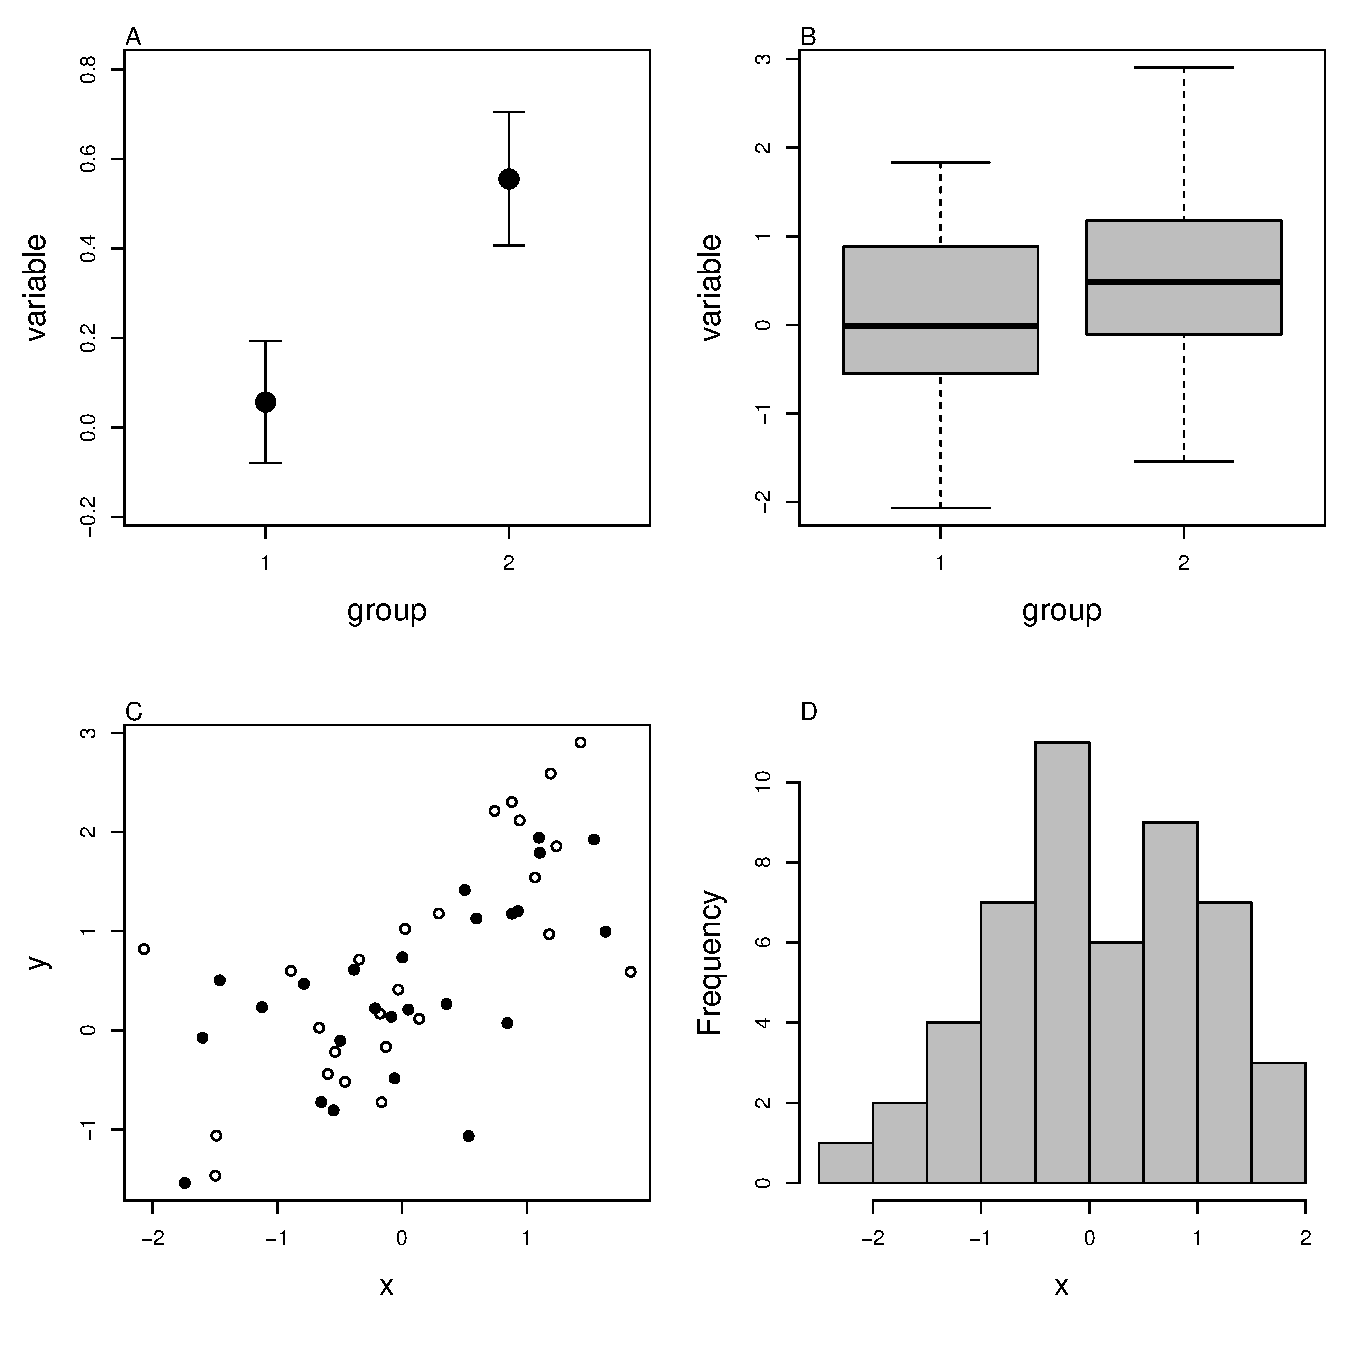
\includegraphics[width=0.75\textwidth]{fig_plot_type.pdf} 
 \caption{Four plot types that \pkg{metaDigitise} is designed to extract data from: A) mean and error plot, B) box plot, C) scatter plot and D) histogram. Data is taken from the iris dataset in R. A and B are plotted with the whole dataset, C and D are just the data for the species setosa.}
\label{fig:plot_type}
\end{figure}

Here, we present an interactive \proglang{R} package, \pkg{metaDigitise}, which is designed for large scale data extraction from figures, specifically catering to the the needs of meta-analysts. To this end, we provide tools specific to data extraction from common plot types (mean and error plots, box plots, scatter plots and histograms, see Figure \ref{fig:plot_type}). \pkg{metaDigitise} operates within the \proglang{R} environment making data extraction, analysis and export more streamlined. 
%% need to be careful abiou th use of the term 'raw data' as internally this means uncalibrated data
It also provides users with options to conduct the necessary calculations on processed data immediately after extraction so that comparable summary statistics can be obtained quickly. \pkg{metaDigitise} condenses summary data extracted from multiple figures into a single data frame which can be can easily be exported. Processed data (i.e., raw data) can also be easily extracted and analysed in any way the user desires in downstream analysis within \proglang{R}. Conveniently, when needing to process many figures at different times \pkg{metaDigitise} will only import figures not already completed within a directory. This makes it easy to add new figures at any time. \pkg{metaDigitise} has also been built for reproducibility in mind. It has functions that allow users to redraw their digitisations on figures, make corrections and access the raw calibration data which is written automatically for each figure that is digitised into a special folder within the directory. This makes sharing figure digitisation and reproducing the work of others simple and easy, and allows meta-analysts to update meta-analyses more easily.




%%%---------------------------------
%%%---------------------------------
%%%---------------------------------



\section{Directory Structure, Image Processing and Reproducibility}

The \pkg{metaDigitise} package is designed to be flexible, yet simple to use. There is one main function in the package, \fct{metaDigitise}, which interactively takes the user through the process of extracting data from figures. \fct{metaDigitise} was created with the idea that the user would likely have multiple images to extract from. It therefore operates in the same way whether the user has one or multiple images. \fct{metaDigitise} is designed to work on a directory containing images of figures copied from primary literature, in .png, .jpg, .tiff, .pdf format. This directory is specified to \fct{metaDigitise} through the \code{dir} argument. The user is free to set their own broad directory structure (e.g. one directory for all images or one directory for each paper extracted from). We would recommend having all files for one project in a single directory with an informative and unambiguous naming scheme for images to make it easy to identify the paper and figure the data come from. This cuts out the need to change directories constantly. For example the directory structure could look like:

\begin{CodeChunk}
\begin{CodeOutput}
* Main project directory
    + FiguresToExtract/
        + Paper1_Figure1_trait1.png
        + Paper1_Figure2_trait2.png
        + Paper1_Figure3_trait3.png
        + Paper2_Figure1_trait1.png
        + Paper2_Figure2_trait2.png
        + Paper2_Figure3_trait3.png
\end{CodeOutput}
\end{CodeChunk}

It is important for the user to think about their directory structure early on in this process (also more generally in the context of their entire project), especially if they plan to share the extractions with collaborators or when publishing the project. 

When \fct{metaDigitise} is run, it recognizes all the images in a directory and automatically imports them one by one, allowing the user to click and enter relevant information about a figure as they go. This expedites digitising figures by preventing users from having to constantly change directories and / or open new images. The data from a completed image is automatically saved in an .RDS file to a \code{caldat} directory, that is created within the parent directory when first executing the \fct{metaDigitise} function. These files enable re-plotting and editing of images at a later point (see below).

A particularly powerful and flexible aspect of \fct{metaDigitise} is its ability to identify images that have been previously digitised and only import images that have not been digitised in subsequent calls of the function. This means that all figures do not need to be extracted at one time and that new figures can be added as the project develops. After each image is extracted, the user is asked whether they wish to continue or quit the extraction process. Upon rerunning \fct{metaDigitise}, previously digitised figures are simply ignored during processing, but their data is re-integrated within the final output after new files are completed automatically.  

After completing all images, or upon quitting, the processed data (in a form specified by the user) is then returned. 
%% how about asking whether summary or not at end? instead of having it in the arguements?
From all plot types, \fct{metaDigitise} summarises the data from a figure as a mean, standard deviation and sample size, for each identified group within the plot (should multiple groups exist). These are the summary statistics needed to create many of the relevant effect sizes and sampling error for a meta-analysis.
%% are there any hwere additional info is needed??
In the case of scatter plots, \fct{metaDigitise} also returns the correlation coefficient between the points within each identified group. 


%%%---------------------------------
%%%---------------------------------
%%%---------------------------------


\section{Diverse Plot Types}
\pkg{metaDigitise} recognises four main types of plot; Mean and error plots, box plots, scatter plots and histograms, shown in Figure \ref{fig:plot_type}. Each of these can be processed together and integrated into a single output. Alternatively, users can keep like figures together and process them separately.


%% where to put calibration???

In order to correctly extract data from figures \fct{metaDigitise} always requires the user to calibrate the axes in the figure. To do this, the user is required to click on two known points on the axis in question, and then enter the value of those points in the figure. Using this information, \fct{metaDigitise} then calculates the value of any clicked points in terms of the figure axes. In the case of mean and error plots and box plots, it calibrates only the y axis (assuming the x axis is redundant). For scatter plots and histograms both axes are calibrated.


\subsection{Mean and error plots} 
\fct{metaDigitise} prompts the user to enter group names and allows the user to enter sample sizes ($n$), which are used in downstream processing. The user is then prompted to click on an error bar followed by the mean. Error bars above or below the mean can be clicked - sometimes one is clearer than the other. \fct{metaDigitise} assumes that the error bars are symmetrical. Where the user has clicked the error is displayed in a different colour to the mean (Figure \ref{fig:all_extract}A). The user can subsequently add more groups, edit groups or remove groups. Finally the user is asked what type of error was used in the figure: standard deviation (SD, $\sigma$), standard error (SE) or 95\% confidence intervals (CI95). Standard deviation is calculated from standard error as
\begin{equation}
\sigma = SE * \sqrt{n}
\end{equation}
and from 95\% confidence intervals as
\begin{equation}
\sigma = \frac{CI}{1.96} * \sqrt{n}
\end{equation}
If the user does not enter a sample size at the time of data extraction (if, for example, the information is not readily available) the SD is not calculated. This can be entered at a later time, however (see below).

\subsection{Box plots}
As with mean and error plots, \fct{metaDigitise} prompts the user to enter group names and allows the user to enter sample sizes ($n$), which are used in downstream processing. The user is then prompted to click on the maximum ($b$), upper quartile ($q_3$), median ($m$), lower quartile ($q_1$) and minimum ($a$). \fct{metaDigitise} will check that the maximum is greater than the minimum, and return a warning if that is not the case. The user can subsequently add, edit or remove groups. From the extracted data, the mean ($\mu$) and SD are calculated as 

\begin{equation}
\mu = \frac{a + 2q_1 + 2m + 2q_3 +b}{8}
\end{equation}

\begin{equation}
\sigma = \frac{b-a}{4\Phi^{-1}(\frac{n-0.375}{n+0.25})} + \frac{q_3-q_1}{4\Phi^{-1}(\frac{0.75n-0.125}{n+0.25})}
\end{equation}

, where $\Phi^{-1}(z)$ is the upper zth percentile of the standard normal distribution, following \citet{Wan2014}. As with mean and error plots, if the user does not enter a sample size at the time of data extraction the SD is not calculated.

\subsection{Scatter plots}
\fct{metaDigitise} prompts the user to enter groups names and then to click on points. Points added by mistake can be deleted. The user can subsequently add groups, edit groups (add or remove points) or delete groups. Different groups are plotted in different colours and shapes, with a legend at the bottom of the figure (Figure \ref{fig:all_extract}C). Mean, SD and sample size (n) are calculated from the clicked points, for each group. Where the sample size from the clicked points does not match a known sample size (e.g. if there are overlaid points), the user can enter an alternate sample size.

\subsection{Histograms}
\fct{metaDigitise} prompts the user to click on the top corners of each bar. Bars can subsequently be deleted. 
For each bar a midpoint (m; mean x coordinates) and a frequency (f; mean y coordinates, rounded to the nearest integer) is calculated. The sample size, mean and SD are calculated as:
\begin{equation}
n = \sum_{i=1}^n{f_i}
\end{equation}

\begin{equation}
\mu = \frac{\sum_{i=1}^n{m_i f_i}}{n}
\end{equation}

\begin{equation}
\sigma = \sqrt{\frac{\sum_{i=1}^n{(m_i f_i - \mu f_i)^2}}{n-1}}
\end{equation}

As with the scatterplots, If the sample size from the extracted data does not match a known sample size, the user can enter an alternate sample size.


\begin{figure}[!h]
\centering 
 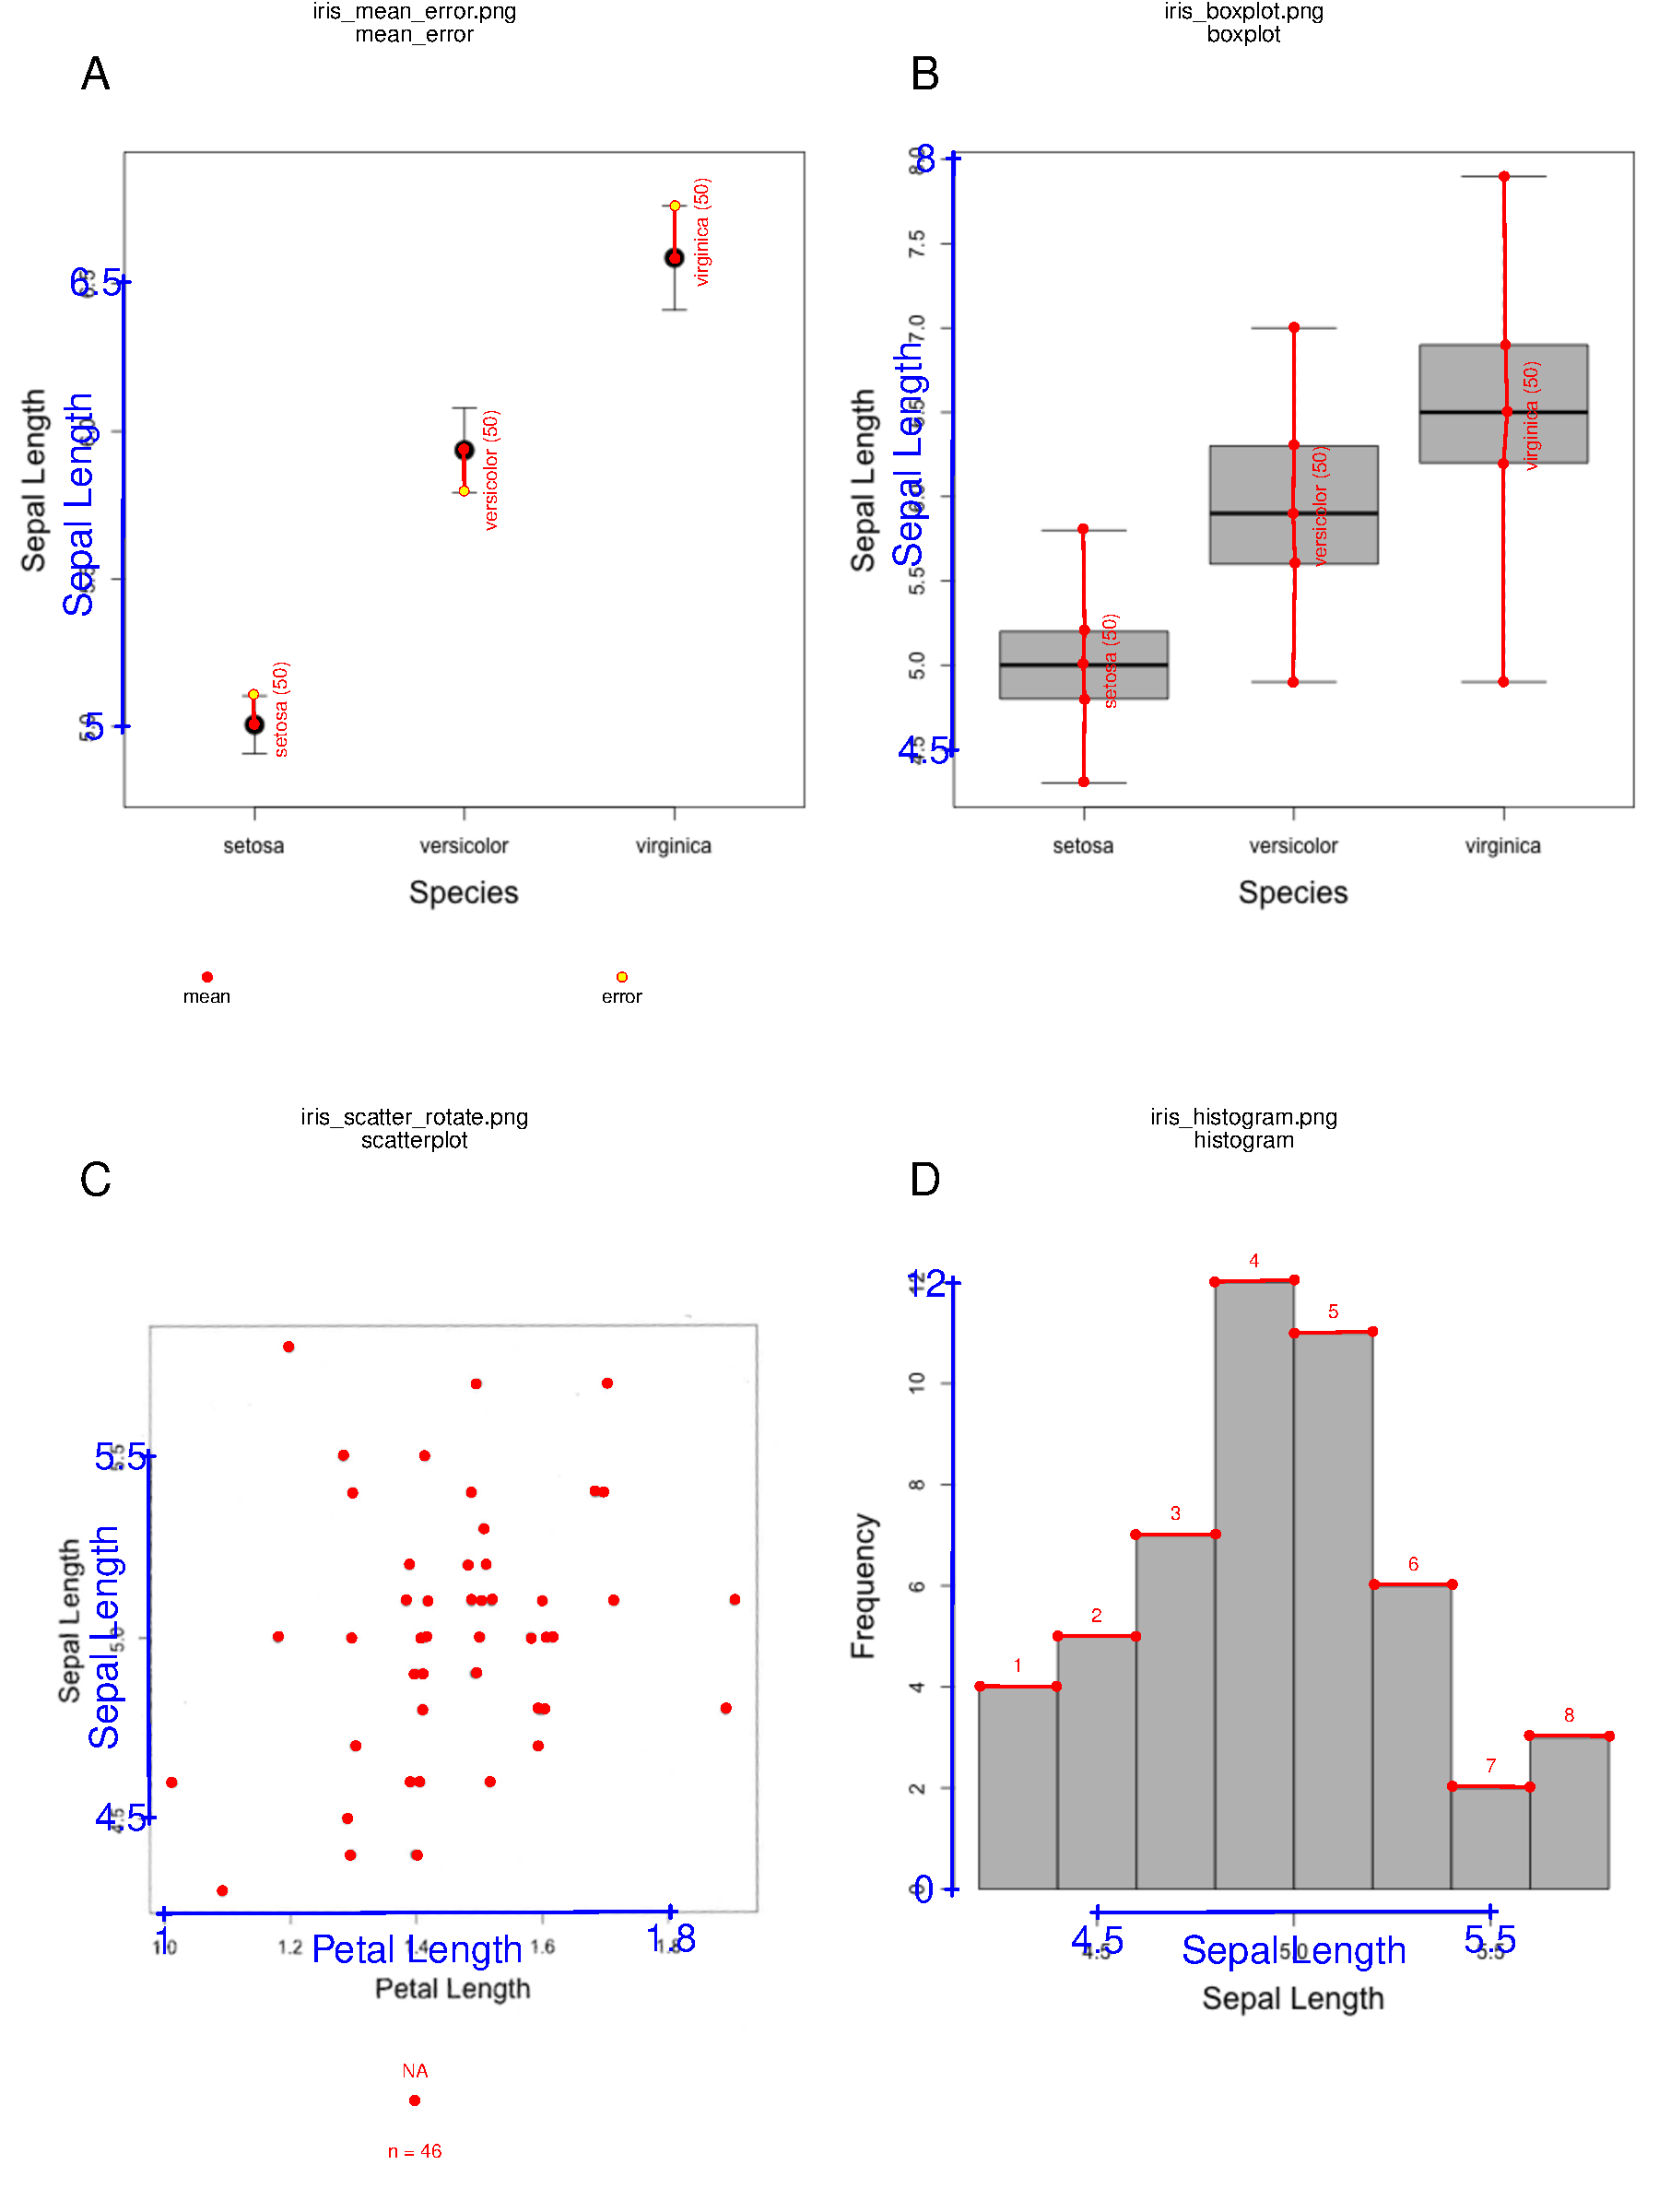
\includegraphics[width=0.75\textwidth]{fig_all_extract.pdf} 
 \caption{Demonstration of data extraction from different plot types}
\label{fig:all_extract}
\end{figure}


%%%---------------------------------
%%%---------------------------------
%%%---------------------------------


\section{Extracting Data From Plots}
%% scatterplot from airquality data


We will now demonstrate how \fct{metaDigitise} works using figures generated from the well known iris data set. Users can install the \pkg{metaDigitise} package from GitHub as follows:

\begin{CodeChunk}
\begin{CodeInput}
R> install.packages("devtools")
R> devtools::install_github("daniel1noble/metaDigitise")
R> library(metaDigitise)
\end{CodeInput}
\end{CodeChunk}

Assume that the user would like to extract summary statistics from studies measuring sepal length or width in iris species for a fictitious project. There are a few studies that only present these data in figures. As the user reads papers found from a systematic search, they add figures with relevant data to a "FiguresToExtract" folder as follows

\begin{CodeChunk}
\begin{CodeOutput}
*FiguresToExtract/
    + 001_Anderson_1935_Fig1.png
\end{CodeOutput}
\end{CodeChunk}

\begin{figure}[!h] 
 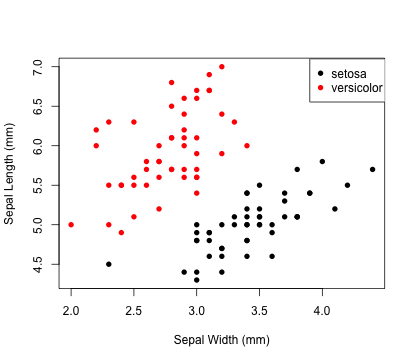
\includegraphics[width=0.75\textwidth]{001_Anderson_1935_Fig1.png} 
 \caption{Example scatterplot (001\_Anderson\_1935\_Fig1.png) of sepal length and width for two species of iris (setosa and versicolor)}
\label{fig:Anderson}
\end{figure}

Here, the naming of the files placed in the folder will contain the paper number, first author and the figure number to keep data uniquely associated with figures. At first there is one figure in the folder, shown in Figure \ref{fig:Anderson}. Running \fct{metaDigitise} brings up a series of prompts for the user using a main menu that provides access to a number of its features: 

\begin{CodeChunk}
\begin{CodeInput}
R> setwd("~/FiguresToExtract")
R> digitised_data <- metaDigitise(".", summary = TRUE)
\end{CodeInput}
\begin{CodeOutput}
	Do you want to...
1: Process new images
2: Import existing data
3: Edit existing data
Selection: 
\end{CodeOutput}
\end{CodeChunk}

The user simply enters in the numeric value that corresponds to what they would like to do. In this case they want to "Process new images". The user is then asked whether there are different types of plot(s) in the folder. This question is most relevant when there are lots of different figures in the folder because it will then ask the user for the type of figure as they are cycled through.

\begin{CodeChunk}
\begin{CodeOutput}
Are all plot types Different or the Same? (d/s)
\end{CodeOutput}
\end{CodeChunk}

\fct{metaDigitise} then asks the user whether the figure needs to be rotated or flipped. This can be needed when box plots and mean and error plots are not orientated correctly. In some cases, older papers can give slightly off angled images which can be corrected by rotating. So, in this prompt the user has three options: \code{f} for "Flip", \code{r} for "rotate" or \code{c} for "continue. 

\begin{CodeChunk}
\begin{CodeOutput}
mean_error and boxplots should be vertically orientated
       _ 
       |  
  I.E. o    NOT  |-o-|
       |
       _

If they are not then chose flip to correct this.

If figures are wonky, chose rotate.

Otherwise chose continue

Flip, rotate or continue (f/r/c) 
\end{CodeOutput}
\begin{CodeInput}
R> c
\end{CodeInput}
\end{CodeChunk}

After this, \fct{metaDigitise} will ask the user to specify the plot type. Depending on the figure, the user can specify that it is a figure containing the mean and error (\code{m}), a box plot (\code
{b}), a scatter plot (\code{s}) or a histogram (\code{h}). If the user has specified \code{diff} instead of \code{same} in response to the question about whether the plot types are the same or different, this question will pop up for each plot, but will only be asked once if plots are all the same.

\begin{CodeChunk}
\begin{CodeOutput}
Please specify the plot_type as either:

 m: Mean and error
 b: Box plot
 s: Scatter plot 
 h: Histogram

 R> s
\end{CodeOutput}
\end{CodeChunk}

After selecting the figure type a new set of prompts will come up that will ask the user first what the y and x-axis variables are. This is useful as users can keep track of the different variables across figures and papers. Here, the user can just add this information in to the \proglang{R} console. Once complete, details on how to calibrate the x and y-axis appear, so that the relevant statistics / data can be correctly calculated. When working with a plot of mean and standard errors, the x-axis is rather useless in terms of calibration so \pkg{metaDigitise} just asks the user to calibrate the y-axis. 

\begin{CodeChunk}
\begin{CodeOutput}
What is the y variable? 
\end{CodeOutput}
\begin{CodeInput}
R> Sepal Length (mm)
\end{CodeInput}

\begin{CodeOutput}
What is the x variable? 
\end{CodeOutput}
\begin{CodeInput}
R> Sepal Width (mm)
\end{CodeInput}

\begin{CodeOutput}
On the Figure, click IN ORDER: 
      y1, y2 , x1, x2  


    Step 1 ----> Click on known value on y axis - y1
  |
  |
  |
  |
  y1
  |_________________________
  ....

    Step 3 ----> Click on known value on x axis - x1
  |
  |
  |
  |
  |
  |_____x1__________________

  ....
\end{CodeOutput}
\end{CodeChunk}

The user can just follow the instructions on screen step-by-step (instructions above have been truncated by `...' to simplify), and in the order specified. Before moving on, the user is forced to check whether or not the calibration has been set up correctly. If \code{n} is chosen because something needs to be fixed then the user can re-calibrate.

\begin{CodeChunk}
\begin{CodeOutput}
What is the value of y1 ?
\end{CodeOutput}
\begin{CodeInput}
R> 4.5
\end{CodeInput}
\begin{CodeOutput}
What is the value of y2 ?
\end{CodeOutput}
\begin{CodeInput}
R> 7
\end{CodeInput}
\begin{CodeOutput}
What is the value of x1 ?
\end{CodeOutput}
\begin{CodeInput}
R> 2
\end{CodeInput}
\begin{CodeOutput}
What is the value of x2 ?
\end{CodeOutput}
\begin{CodeInput}
R> 4
\end{CodeInput}
\begin{CodeOutput}
Re-calibrate? (y/n) 
R> n
\end{CodeOutput}
\end{CodeChunk}

Often, plots might contain multiple groups that the meta-analyst wants to extract from. \fct{metaDigitise} handles this nicely by prompting the user to enter the group first, followed by digitisation of this groups data. After digitising the first group, and having exited (e.g., hit `esc' on mac from plot window), \fct{metaDigitise} will ask the user whether they would like to add another group. Users can continually add groups (\code{a}), delete groups (\code{d}), edit groups (\code{e}) or finish a plot and continue to the next one (\code{f} - if another plot exists). 
%%% This needs checking - think it is now different
The number of groups are not really limited and users can just keep adding in groups to accommodate the different numbers that may be presented across figures (although it can get complicated with too many).

\begin{CodeChunk}
\begin{CodeOutput}
Follow instructions below, to exit point adding or removing:

 - Windows: right click on the plot area and choose 'Stop'!

 - X11: hit any mouse button other than the left one.

 - quartz/OS X: hit ESC

Group identifier:
\end{CodeOutput}
\begin{CodeInput}
R> setosa
\end{CodeInput}
\begin{CodeOutput}
Click on points you want to add.
If you want to remove a point, or are finished with a
group, exit (see above), then follow prompts

Add points, delete points or continue? (a/d/c) 
\end{CodeOutput}
\begin{CodeInput}
R> c
\end{CodeInput}
\end{CodeChunk}

Once we are done digitising all the groups our plot will look something like Figure \ref{fig:scatter_extract}

\begin{figure}[!h] 
 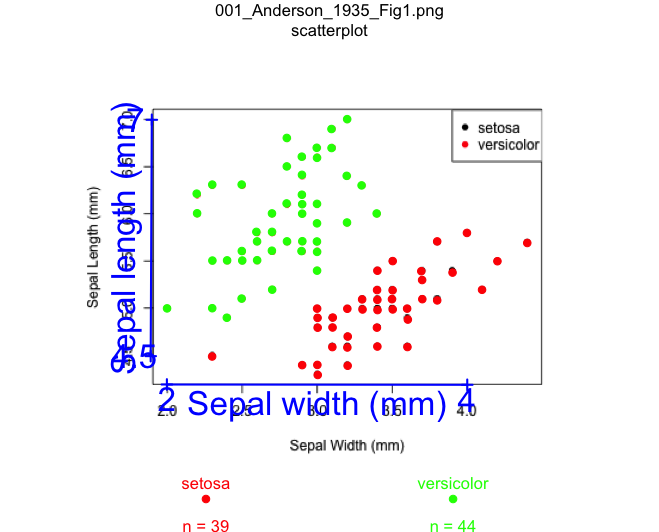
\includegraphics[width=0.9\textwidth]{001_Anderson_1935_Fig1_digitised.png} 
 \caption{Digitisation of sepal length and width for two species of iris (setosa and versicolor). Names of the variables and calibration (in blue) are plotted alongside the digitised points (green = versicolor; red = setosa). The sample sizes for each group are provided on the lower part of the plot. All figures are clearly labeled at the top to remind users of the filename and plot type. This reduces errors throughout the digitisation process.}
\label{fig:scatter_extract}
\end{figure}

When completed \pkg{metaDigitise} will write the digitised data to the caldat directory, such that our new directory structure is as follows

\begin{CodeChunk}
\begin{CodeOutput}
*FiguresToExtract/
    + caldat/
        + 001_Anderson_1935_Fig1
    + 001_Anderson_1935_Fig1.png
\end{CodeOutput}
\end{CodeChunk}

Users can access the \pkg{metaDigitise} object created (001\_Anderson\_1935\_Fig1) at any time using the metaDigitse function. In the \proglang{R} console, the summarised data for the digitised figure can be printed on screen or even written to a .csv file:

\begin{CodeChunk}
\begin{CodeInput}
R> digitised_data
\end{CodeInput}
\begin{CodeOutput}
                  filename    group_id         variable  mean  error error_type  n     r    sd  plot_type
001_Anderson_1935_Fig1.png      setosa  Sepal width (mm)  3.42  0.40  sd        39  0.75  0.40  scatterplot
001_Anderson_1935_Fig1.png      setosa  Sepal length (mm) 5.00  0.38  sd        39  0.75  0.38  scatterplot
001_Anderson_1935_Fig1.png  versicolor  Sepal width (mm)  2.77  0.32  sd        44  0.52  0.32  scatterplot
001_Anderson_1935_Fig1.png  versicolor  Sepal length (mm) 5.95  0.53  sd        44  0.52  0.53  scatterplot
\end{CodeOutput}
\end{CodeChunk}

The mean for each of the two variables, along with the two species, are provided. Since this is a scatterplot, the user also gets the Person's correlation coefficient between sepal length and width for each species. These match reasonably well with the actual means of sepal length and width for each of the species in the full `iris` dataset:

\begin{CodeChunk}
\begin{CodeOutput}
     Species meanSL meanSW
1     setosa  5.006  3.428
2 versicolor  5.936  2.770
\end{CodeOutput}
\end{CodeChunk}

One thing anyone with a familiarity with the iris dataset will notice is that the sample sizes for each of these species (which are n = 50 each) are quite a bit lower. This is an example of some of the challenges when extracting data from scatter plots. Often data points will overlap with each other making it impossible (without having the real data) to know whether this is a problem. However, a meta-analyst will probably realise that the sample sizes here conflict with what is reported in the paper. Hence, \pkg{metaDigitise} also provides the user with  options to input the sample sizes directly (see Editing section below), even for scatter plots and histograms where, strictly speaking, this should not be necessary. Nonetheless, it is important to recognise the impact that overlapping points can have on summary statistics, particularly its effects on standard deviation (SD) and standard error (SE). Here, the mean point estimates are nearly bang on, but the SD's are slightly over-estimated:

\begin{CodeChunk}
\begin{CodeOutput}
     Species    meanSL    meanSW
1     setosa 0.3524897 0.3790644
2 versicolor 0.5161711 0.3137983
\end{CodeOutput}
\end{CodeChunk}



\subsection{Adding new figures}

Users can add additional figures as new papers with relevant information are found. Each figure should be in its own file with unique naming, even if a single paper has multiple figures for extraction. For example, another paper on different populations (and one new species) of iris contained two additional figures where important data could be extracted. These figures can simply be named accordingly and added directly to the same extraction folder: 

\begin{CodeChunk}
\begin{CodeOutput}
*FiguresToExtract/
	+ caldat/
	  	+ 001_Anderson_1935_Fig1
    + 001_Anderson_1935_Fig1.png
    + 002_Doe_2013_Fig1.png
    + 002_Doe_2013_Fig3.png
\end{CodeOutput}
\end{CodeChunk}

The user has already processed one figure (001\_Anderson\_1935\_Fig1.png). We can tell this because the caldat folder has digitised data in it (caldat/001\_Anderson\_1935\_Fig1). Now the user has two new figures that have not yet been digitised. This example will nicely demonstrate how users can easily pick up from where they left off and how all previous data gets re-integrated. It will also demonstrate how different plot types are handled. All we have to do to begin, is again, provide the directory where all the figures are located:

\begin{CodeChunk}
\begin{CodeInput}
R> setwd("~/FiguresToExtract")
R> digitised_data <- metaDigitise(".", summary = TRUE)
\end{CodeInput}
\end{CodeChunk}

The user gets the same set of prompts and simply chooses option one. This will permit users to digitise new figures, and will integrate previously completed digitisations along with newly digitised data together at the end of the session, or when the user decides to quit. This time, 001\_Anderson\_1935\_Fig1.png, is ignored and the new plots cycle on screen. First for 002\_Doe\_2013\_Fig1.png and then 002\_Doe\_2013\_Fig3.png. Since there are a few different figure types, the user answers the first question in the \proglang{R} console as "diff":

\begin{CodeChunk}
\begin{CodeOutput}
Are all plot types the same? (diff/same) 
\end{CodeOutput}
\begin{CodeInput}
R> diff
\end{CodeInput}
\begin{CodeOutput}
**** NEW PLOT ****

mean_error and boxplots should be vertically orientated
       _ 
       |  
  I.E. o    NOT  |-o-|
       |
       _

If they are not then chose flip to correct this.

If figures are wonky, chose rotate.

Otherwise chose continue

Flip, rotate or continue f/r/c 
\end{CodeOutput}
\begin{CodeInput}
R> c
\end{CodeInput}
\begin{CodeOutput}
Please specify the plot_type as either: mean and error, box plot,
scatter plot or histogram m/b/s/h: 
\end{CodeOutput}
\begin{CodeInput}
R> m
\end{CodeInput}
\end{CodeChunk}

Here, the user specifies the new plot type as \code{m} for 002\_Doe\_2013\_Fig1.png because the user has a plot of the mean and error of sepal length for each of the three species. The user is then prompted a bit differently from our scatter plot as the x-axis is not needed for calibration:

\begin{CodeChunk}
\begin{CodeOutput}
What is the variable? 
\end{CodeOutput}
\begin{CodeInput}
R> Sepal length
\end{CodeInput}
\begin{CodeOutput}
On the Figure, click IN ORDER: 
      y1, y2  


    Step 1 ----> Click on y1
  |
  |
  |
  |
  y1
  |_________________________


    Step 2 ----> Click on y2
  |
  y2
  |
  |
  |
  |_________________________
  
What is the value of y1 ?
\end{CodeOutput}
\begin{CodeInput}
R> 5
\end{CodeInput}
\begin{CodeOutput}
What is the value of y2 ?
\end{CodeOutput}
\begin{CodeInput}
R> 6.5
\end{CodeInput}
\begin{CodeOutput}
Re-calibrate? (y/n) 
\end{CodeOutput}
\begin{CodeInput}
R> n
\end{CodeInput}
\begin{CodeOutput}
Enter sample sizes? y/n 
\end{CodeOutput}
\begin{CodeInput}
R> y
\end{CodeInput}
\begin{CodeOutput}
Group identifier: 
\end{CodeOutput}
\begin{CodeInput}
R> setosa
\end{CodeInput}
\begin{CodeOutput}
Group sample size: 
\end{CodeOutput}
\begin{CodeInput}
R> 50
\end{CodeInput}
\begin{CodeOutput}
Click on Error Bar, followed by the Mean

Add group, Delete group or Finish plot? a/d/f 
\end{CodeOutput}
\begin{CodeInput}
R> a
\end{CodeInput}
\end{CodeChunk}

Again, \fct{metaDigitise} will simply guide the user through digitising each of these figures describing to them exactly what needs to be done. At any point if mistakes are made the user can choose relevant options to edit or correct things before ending the figure. This process continues for each plot so long as the user would like to continue and after completing a single plot the user is always prompted as follows:

\begin{CodeChunk}
\begin{CodeOutput}
Do you want continue: 1 plots out of 2 plots remaining (y/n)
\end{CodeOutput}
\begin{CodeInput}
R> y
\end{CodeInput}
\end{CodeChunk}

This continues until users have completed all non-digitised figures in the folder, at which point \fct{metaDigitise} concatenates the new data with previously digitised data in the object:

\begin{CodeChunk}
\begin{CodeOutput}
data
                  filename    group_id         variable   mean  error error_type n    r    sd   plot_type
001_Anderson_1935_Fig1.png      setosa  Sepal width (mm)  3.42  0.40  sd        39  0.75  0.40  scatterplot
001_Anderson_1935_Fig1.png      setosa  Sepal length (mm) 5.00  0.38  sd        39  0.75  0.38  scatterplot
001_Anderson_1935_Fig1.png  versicolor  Sepal width (mm)  2.77  0.32  sd        44  0.52  0.32  scatterplot
001_Anderson_1935_Fig1.png  versicolor  Sepal length (mm) 5.95  0.53  sd        44  0.52  0.53  scatterplot
     002_Doe_2013_Fig1.png      setosa  Sepal length      5.00  0.11  se        50  NA    0.78  mean_error
     002_Doe_2013_Fig1.png  viriginica  Sepal length      6.59  0.18  se        50  NA    1.26  mean_error
     002_Doe_2013_Fig1.png  versicolor  Sepal length      5.94  0.14  se        50  NA    1.01  mean_error
     003_Doe_2013_Fig3.png      catana  Sepal length      4.95  0.36  sd        50  NA    0.36  histogram
\end{CodeOutput}
\end{CodeChunk}


\section{Re-importing, Editing and Plotting Previously Digitised data}

A particularly useful feature of \pkg{metaDigitise} is its ability to re-import, edit and re-plot previously digitised figures. We can do this from the initial options from \fct{metaDigitise}


\begin{CodeChunk}
\begin{CodeInput}
R> setwd("~/FiguresToExtract")
R> digitised_data <- metaDigitise(".")
\end{CodeInput}
\begin{CodeOutput}
    Do you want to...
1: Process new images
2: Import existing data
3: Edit existing data
Selection: 
\end{CodeOutput}
\end{CodeChunk}

If the user chooses "Import existing data", they have the option of either 1) importing data from all digitised images or 2) importing data from particular image that has been digitised. If 2, then a list of files are provided to the user that they can select. Editing existing data allows users to easily re-plot or edit information or digitisations that have previously be done for any plot. This is accomplished by guiding the user through a new set of options:

\begin{CodeChunk}
\begin{CodeOutput}
Choose how you want to edit files:
1: Cycle through images
2: Choose specific file to edit
3: Enter previously omitted sample sizes
Selection: 
\end{CodeOutput}
\end{CodeChunk}

If the user is unsure about the name of the specific figure they need to edit or simply want to just check the digitisations of figures they can choose "Cycle through images", which will bring up each figure, one by one, overlaying the calibrations, group names (if they exist), sample sizes (if they were entered) and the selected points. The user will then be given the choice to edit individual images. Alternatively, choosing option 2, will bring up a list of the completed files in the folder and the specific file can be chosen, at which point it will be replotted. Either of these options will cycle through a number of questions asking the user what they would like to edit:

\begin{CodeChunk}

\begin{CodeOutput}
Edit rotation? If yes, then the whole extraction will be redone (y/n) 
\end{CodeOutput}
\begin{CodeInput}
R> n
\end{CodeInput}
\begin{CodeOutput}
Change plot type? If yes, then the whole extraction will be redone (y/n) 
\end{CodeOutput}
\begin{CodeInput}
R> n
\end{CodeInput}
\begin{CodeOutput}
Variable entered as: 
\end{CodeOutput}
\begin{CodeInput}
R> Sepal length
\end{CodeInput}
\begin{CodeOutput}
Rename Variables (y/n) 
\end{CodeOutput}
\begin{CodeInput}
R> n
\end{CodeInput}
\begin{CodeOutput}
Edit calibration? (y/n) 
\end{CodeOutput}
\begin{CodeInput}
R> n
\end{CodeInput}
\begin{CodeOutput}
Re-extract data (y/n) 
\end{CodeOutput}
\begin{CodeInput}
R> y
\end{CodeInput}
\begin{CodeOutput}
Change group identifier? (y/n) 
\end{CodeOutput}
\begin{CodeInput}
R> n
\end{CodeInput}
\begin{CodeOutput}
Add group, Delete group or Finish plot? (a/d/f) 
\end{CodeOutput}
\begin{CodeInput}
R> d
\end{CodeInput}
\begin{CodeOutput}
1: setosa
2: versicolor
3: viriginica
Selection: 
\end{CodeOutput}
\begin{CodeInput}
R> 2
\end{CodeInput}
\begin{CodeOutput}
Add group, Delete group or Finish plot? (a/d/f) 
\end{CodeOutput}
\begin{CodeInput}
R> a
\end{CodeInput}

\end{CodeChunk}

A whole host of information can be edited including the rotation, plot type, the variable name(s) that were provided, the calibration and even the digitisation of groups. When editing the \code{metaDigitise} object is re-written to the caldat folder and the edits are immediately integrated into the existing object once complete. 


\section{Additional Features}

\subsection{Figure Rotation and Adjustment}
Figures may have been extracted from old publications, for example from scanned images, and so are not perfectly orientated on the image. This will make the calibration of the points in the figure from the image problematic. \fct{metaDigitise} allows users to rotate the image. By clicking two points on the x-axis, metaDigitse calculates the angle needed to rotate the image so the x-axis is horizontal, and rotates it. (Figure \ref{fig:rotate}A,B)

\begin{figure}[!b] 
 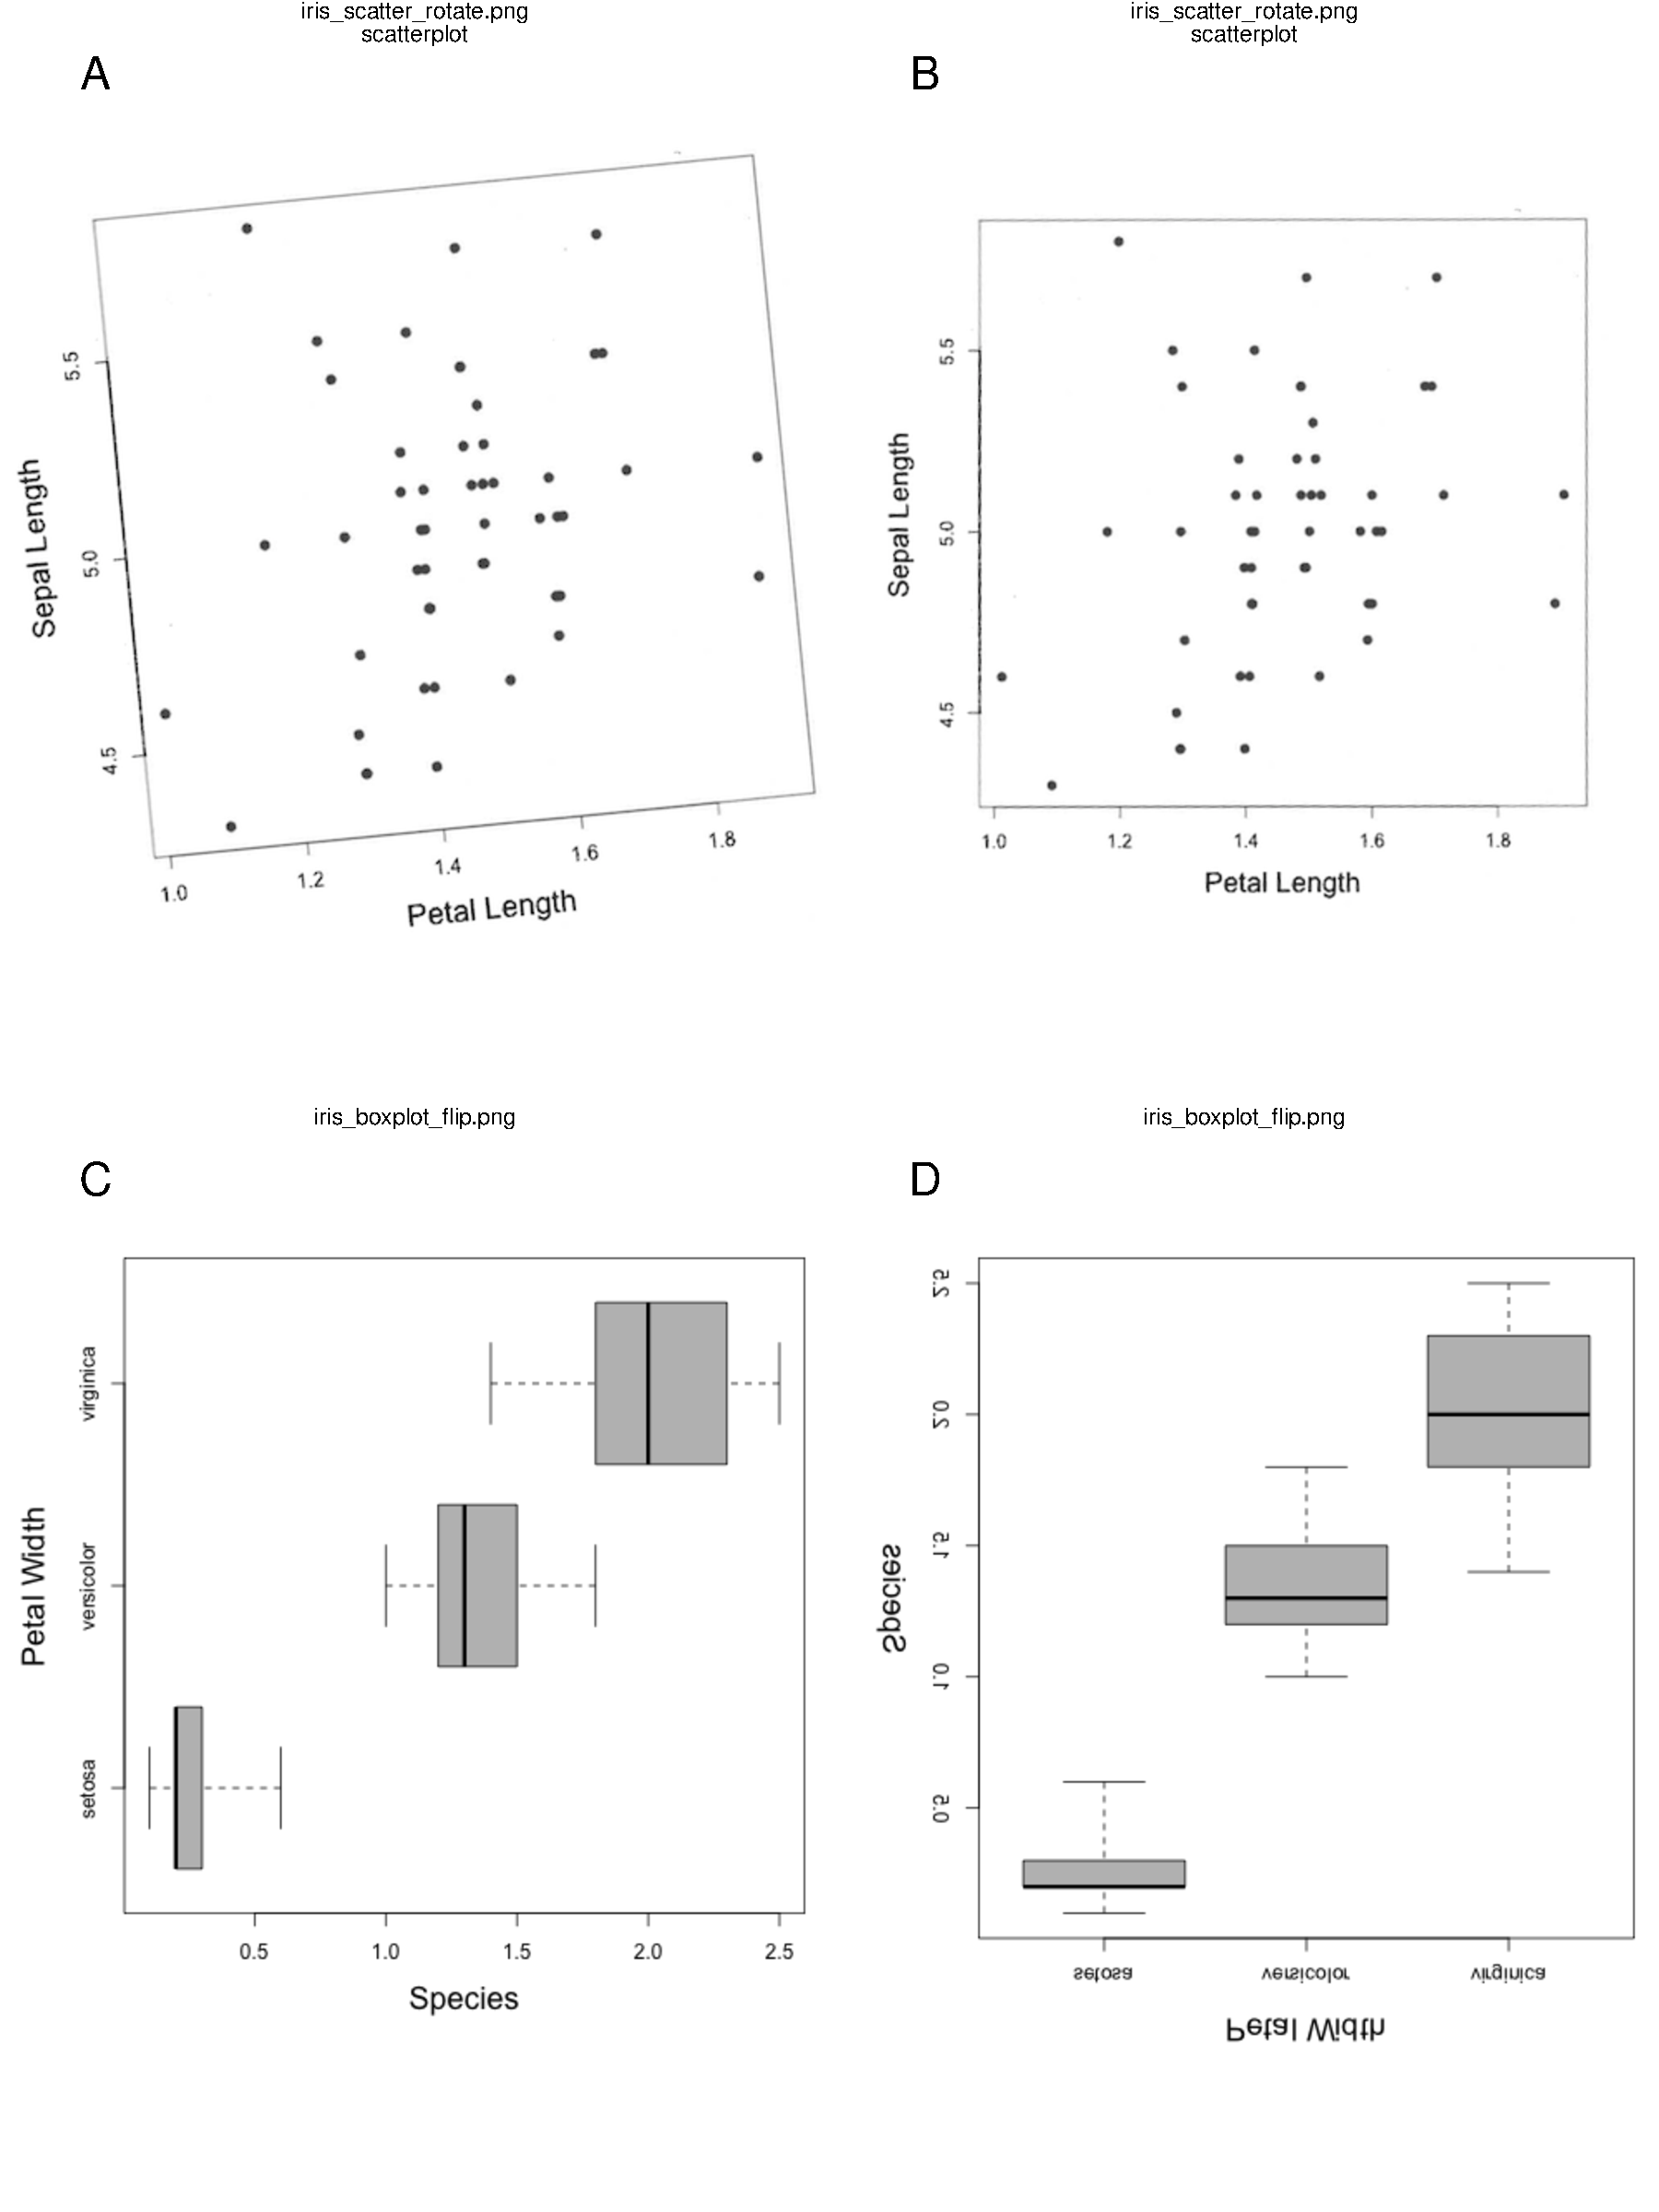
\includegraphics[width=0.9\textwidth]{fig_rotate.pdf} 
 \caption{Figure rotation. A) and B) show how non-aligned images can be realigned through user defined rotation. C) and D) show how figures can be re-orientated so as to aid data input.}
\label{fig:rotate}
\end{figure}

Furthermore, some figures, including mean and error, boxplots or histograms, may be presented with horizontal bars. \fct{metaDigitise} assumes that the bars are vertical, but allows the user to flip the image so that the bars are vertical if provided horizontally (Figure \ref{fig:rotate}C,D).

\subsection{Obtaining Processed Data}

While \fct{metaDigitise} provides users with the summary statistics by default, for all plot types, in many cases the user may actually be interested in obtaining the processed digitised data from scatter plots (i.e. calibrated points). This is very easy to do my changing the default \code{summary} argument from TRUE to FALSE in \fct{metaDigitise}. Instead of providing the user with summary statistics it will return a list containing four slots for each of the figure types (mean error, box plot, histogram and scatter plots). An example of a data object returned from digitising figures is as follows:

\begin{CodeChunk}

\begin{CodeInput}
>R str(data)
\end{CodeInput}

\begin{CodeOutput}
List of 3
 $ mean_error :List of 1
  ..$ 002_Doe_2013_Fig1.png:'data.frame': 3 obs. of  5 variables:
  .. ..$ id      : Factor w/ 3 levels "setosa","versicolor",..: 1 2 3
  .. ..$ mean    : num [1:3] 5 5.93 6.59
  .. ..$ error   : num [1:3] 0.111 0.148 0.178
  .. ..$ n       : num [1:3] 50 50 50
  .. ..$ variable: chr [1:3] "Sepal length" "Sepal length" "Sepal length"
 $ hist       :List of 1
  ..$ 003_Doe_2013_Fig3.png:'data.frame': 8 obs. of  3 variables:
  .. ..$ midpoints: num [1:8] 4.3 4.5 4.7 4.9 5.1 ...
  .. ..$ frequency: num [1:8] 4 5 7 12 11 6 2 3
  .. ..$ variable : chr [1:8] "Sepal length" "Sepal length" ...
 $ scatterplot:List of 1
  ..$ 001_Anderson_1935_Fig1.png:'data.frame':  83 obs. of  8 variables:
  .. ..$ id        : Factor w/ 2 levels "setosa","versicolor": 1 1 1 1 1 ...
  .. ..$ x         : num [1:83] 2.3 2.9 3 3 3 ...
  .. ..$ y         : num [1:83] 4.5 4.4 4.41 4.3 4.8 ...
  .. ..$ group     : num [1:83] 1 1 1 1 1 1 1 1 1 1 ...
  .. ..$ col       : Factor w/ 2 levels "red","green": 1 1 1 1 1 1 1 1 1 ...
  .. ..$ pch       : num [1:83] 19 19 19 19 19 19 19 19 19 19 ...
  .. ..$ y_variable: chr [1:83] "Sepal length (mm)" "Sepal length (mm)"  ...
  .. ..$ x_variable: chr [1:83] "Sepal width (mm)" "Sepal width (mm)"    ...
\end{CodeOutput}
\end{CodeChunk}

Here, the user can easily access the list of processed scatter plot data by simply extracting the scatter plot slot:

\begin{CodeChunk}
\begin{CodeInput}
>R scatterplot <- data$scatterplot
\end{CodeInput}
\end{CodeChunk}

\subsection{Adding sample sizes to previous Digitisations}
%Including addition of N later
In many cases important information, such as sample sizes, may not be readily available or clear when digitising figures. In these circumstances users will have answered 'no' to the question about whether they have sample sizes or not while digitising. To expedite finding and adding in these sample sizes to do the necssary calculations (if for example a figure presented 95\% CI's or standard errors), \pkg{metaDigitise} has s specific edit option that allows users to enter in previously omitted sample sizes. It works by first identifying the missing sample sizes in the digitised output, re-plotting the relevant figure and then prompting the user to enter the sample sizes for the relevant groups in the figure, 1 by one. As an example, assume that we were missing sample sizes for two groups in 002\_Doe\_2013\_Fig1.png:

\begin{CodeChunk}
\begin{CodeOutput}
                  filename    group_id         variable   mean  error error_type n    r    sd   plot_type
     002_Doe_2013_Fig1.png      setosa  Sepal length      5.00  0.11  se        NA  NA    NA  mean_error
     002_Doe_2013_Fig1.png  viriginica  Sepal length      6.59  0.18  se        NA  NA    NA  mean_error
\end{CodeInput}
\end{CodeChunk}

Here, we can see that we are missing the sample sizes for setosa and viriginica, and as a result, sd is not calculated because \pkg{metaDigitise} needs this information to make the calculation. If the user found this information after contacting the authors for clarification then they can add these back in as follows:

\begin{CodeChunk}
\begin{CodeInput}
>R setwd("~/FiguresToExtract")
>R digitised_data <- metaDigitise(".")
\end{CodeInput}
\end{CodeChunk}

\begin{CodeChunk}
\begin{CodeInput}
Do you want to...

1: Process new images
2: Import existing data
3: Edit existing data

Selection: 3
\end{CodeInput}
\end{CodeChunk}

\begin{CodeChunk}
\begin{CodeInput}
Choose how you want to edit files:

1: Cycle through images
2: Choose specific file to edit
3: Enter previously omitted sample sizes

Selection: 3
\end{CodeInput}
\end{CodeChunk}

\pkg{metaDigitise} will replot the figure after this and list, only the groups missing data, for which the user can then update the data. This is then re-integrated back into the data automatically and the sd calculated. 

\begin{CodeChunk}
\begin{CodeInput}
Group " setosa ": Enter sample size  
50

Group " viriginica ": Enter sample size  
50
\end{CodeInput}
\end{CodeChunk}

\section{Interobserver Variability and Validation}
%% simulated data
%% x people doing y plots
\subsection{Interobserver variability in digitisations}
We evaluated the consistency of digitisation using \pkg{metaDigitise} by simulating a dataset with two different groups and two traits. These data were then used to construct four different plot types (scatterplot, mean and error, histogram and boxplots). Each variable was plotted twice for a given plot type (figures were modified slightly to give users a sense that they were digitising new data) generating a total of 14 figures. We randomised the order of these figures (using the same data) and provided the entire figure directory to a total of 15 indpendent digitisers. The same data was presented at least twice for each figure type to estimate between- and within- user variability (i.e., the intra-class correlation coefficient) in the data. Digitisers varied in their level of experience from those having done meta-analyses or comparative work to those not having any experience doing so. We got users to digitise all 14 figures and then send the data on these to evaluate interobserver variablity across the plots. 

We analysed these data by first transformting each users mean, standard deviation and correlation coefficient generated from their digitisations to standardized mean differences (in otherwords, deviations were percentage differences from the true summary statistics). We then estimated intra-class correlation coefficients (ICC) (adjusted - accounting for covariates and unadjusted - not accounting for covariates) using linear mixed effect models with user identify as a random effect. We tested the significance of ICC estimates using liklihood ratio tests based on 1000 parametric bootstraps of the model. The overall model also included plot type, variable and group to account for possible biases across the variables and plots. We used standardised mean, standard deviation and correlation coeficients as response variables in seperate models using both \pkg{lme4} \citep{bates2015} and \pkg{MCMCglmm} \citep{hadfield2010}, estimating ICC using the \pkg{rptR} package \citep{stoffel2017} in R. If digitisations were consistent across all users then we would predict no significant between user variability in the data. 

\subsection{Testing the accuracy of digitisations}
To test how accurate \pkg{metaDigitise} is at matching points to their true values, we generated four random scatterplots and tested how well the digitised point in each scatterplot matches the actual, true point generated from simulations. We evaluated the accuracy using a Pearson's correlation coefficient between the digitised data from \pkg{metaDigitise} and the true known data value from the simulated data. 


\subsection{Results}

Across plot types we found no evidence for any inter-observer variability in digitisations for the mean (Unadjusted ICC = 0, 95\% CI = 0 to 0.029, p = 1; Adjusted ICC = 0, 95\% CI = 0 to 0.033, p = 1), standard deviation (Unadjusted ICC = 0, 95\% CI = 0 to 0.033, p = 0.5; Adjusted ICC = 0.002, 95\% CI = 0 to 0.032, p = 1) or correlation coefficient (Unadjusted ICC = 0.053, 95\% CI = 0 to 0.296, p = 0.377; Adjusted ICC = 0.048, 95\% CI = 0 to 0.3, p = 0.374). Overall, there were very small differences between digitised values and the true values only deviating, on average 3.34\% (mean = 0.02\%, sd = 5\%, r = 5\%) for all three summary statistics.
%% Note that unadjusted and adjusted values come from rptR and the deviation of percent are the intercept values (*100) for mean, sd and r. I've averaged these three for 3.34% 

Digitised data was essentially perfectly correlated with the true simulated data for both the x-variable (r = 0.9999915, t = 2137.4, df = 78, p-value < 2.2e-16) and y-variable (r = 0.9999892, t = 1897.8, df = 78, p-value < 2.2e-16) in scatterplots.  

\section{Discussion and Conclusions}

%% discuss specifically everything it can't do, and jsutify it slightly

\begin{sidewaystable}[t!]
{\centering
\begin{tabular}{lccccccc}
\hline
Function                  & metaDigitise & GraphClick$^1$ & DataThief$^2$  & DigitizeIt$^3$ & WebPlotDigitizer$^4$ & metagear$^5$ & digitize$^6$\\
\hline
Scatterplots              & \checkmark   & \checkmark & \checkmark & \checkmark & \checkmark     & \checkmark$^7$ & \checkmark \\
Mean and error plots      & \checkmark   & \checkmark & \checkmark & $\times$   & $\times$       & \checkmark$^7$ & $\times$    \\
Boxplots                  & \checkmark   & $\times$   & $\times$   & $\times$   & $\times$       & $\times$       & $\times$    \\
Histograms                & \checkmark   & $\times$   & $\times$   & $\times$   & \checkmark$^7$ & $\times$       & $\times$    \\
Graph rotation$^8$        & \checkmark   & \checkmark & \checkmark & \checkmark & \checkmark     & $\times$       & $\times$    \\
Groups                    & \checkmark   & \checkmark & $\times$   & \checkmark & \checkmark     & $\times$       & $\times$    \\
Entry of metadata         & \checkmark   & $\times$   & $\times$   & $\times$   & $\times$       & $\times$       & $\times$    \\
Summarising data          & \checkmark   & $\times$   & $\times$   & $\times$   & $\times$       & $\times$       & $\times$    \\
Multiple image processing & \checkmark   & $\times$   & $\times$   & $\times$   & $\times$       & $\times$       & $\times$    \\
Reproducable$^9$  & \checkmark   & \checkmark & \checkmark & $\times$   & \checkmark     & $\times$       & $\times$    \\
Automated point detection & $\times$     & \checkmark &     ?      & \checkmark & \checkmark     & \checkmark     & $\times$    \\
Line extraction           & $\times$     & \checkmark & \checkmark & \checkmark & \checkmark     & $\times$       & $\times$    \\
Zoom                      & $\times$     & \checkmark & \checkmark & \checkmark &       ?        & $\times$       & $\times$    \\
Log axis                  & $\times$ *   & \checkmark & \checkmark & \checkmark & \checkmark     & $\times$       & $\times$    \\
Dates                     & $\times$ *   & $\times$   & \checkmark & $\times$   & \checkmark     & $\times$       & $\times$    \\
Asymmetric error bars     & $\times$     & $\times$   & \checkmark & $\times$   & $\times$       & $\times$       & $\times$    \\
Freeware                  & \checkmark$^{10}$ & \checkmark$^{11}$ & \checkmark$^{11}$ & $\times$$^{11}$ & \checkmark$^{11}$ & \checkmark$^{10}$ & \checkmark$^{10}$\\
\hline

%http://datathief.org/DatathiefManual.pdf
%http://www.digitizeit.de/#Features
%https://automeris.io/WebPlotDigitizer/userManual.pdf

\end{tabular}
}
{\footnotesize
\\
$^1$ \citet{GraphClick}
$^2$ \citet{DataThief}
$^3$ \citet{DigitizeIt}
$^4$ \citet{WebPlotDigitizer}
$^5$ \citet{Lajeunesse2016}
$^6$ \citet{Poisot2011}
\\$^7$ Only automated, no manual extraction.
\\$^8$ Or handles rotated graphs. 
\\$^9$ Allows saving, re-plotting and editing of data extraction.
\\$^{10}$ \proglang{R} package.
\\$^{11}$ Standalone software.
}

\caption{\label{tab:comparison} Comparison of functionality between different digitisation softwares.}

\end{sidewaystable}


Although \pkg{metaDigitise} is already very flexible, and provides functionality not seen in any other packages (Table \ref{tab:comparison}) it is clear that there are some functions that it does not perform. A notable feature that \pkg{metaDigitise} lacks is automated point detection. This is available in several packages (Table \ref{tab:comparison}). However, from our experience of using these functions, manual digitising is more reliable and often equally as fast. Particularly given that calibration (for point detection) needs to be done for each plot individually in any case. Additionally, auto-detection often misses many points which then subsequently need to be manually added. Bssed on tests of \pkg{metaDigitise} (see above) figures can be extracted in around 1-2 minutes, including the entry of metadata. As a result, we do not belive that current automated point detection provides substantial time saving benefits.

Another feature that \pkg{metaDigitise} (currently) lacks, is an ability to zoom in plots. This may enable users to gain greater accuracy when clicking on points. However, from our own experience (and indeed the results from our inter-observer reliability), if you are using a reasonably sized screen then the accuracy is already high from these programs (see results above for example), and there is not much gain is to be had from zooming in on points in many circumstances.

In contrast to some other packages, \pkg{metaDigitise} currently also does not extract lines from figures. In our own experience, this is not particularly useful for meta-analysis, although we recognise that it may be useful in other fields. In this case, we would recommend extracting data as a scatter plot, and clicking along the line in question. A model can then be fitted to these points to estimate the parameters needed.

Finally, \pkg{metaDigitise} currently also does not allow for asymmetric error bars. At present this is a deliberate omission, as it is not clear how best to derive SD from such data, given also that such asymmetric error bars may represent different things in different figures. 

Increasing the reproducibility of figure extraction for meta-analysis and making the laborious process more streamlined, flexible and integrated with existing statistical software will go a long way in facilitating the production of high quality meta-analytic studies that can be updated in the future. We belive that \pkg{metaDigitise} will improve this research synthesis pipeline, and will hopefully become an integral package that can be added to the meta-analysts toolkit.


\section*{Acknowledgments}
We thank the I-DEEL group at UNSW for increadibly useful feedback, and a host of colleagues for testing, providing feedback and digitising including: Rose O'Dea, Fonti Kar, Malgorzata Lagisz, Julia Riley, Diego Barneche, Erin Macartney, Ivan Beltran, Gihan Samarasinghe, Dax Kellie, Jonathan Noble and Yian Noble. DWAN was supported by an Australian Research Council Discovery Early Career Research Award (DE150101774) and UNSW Vice Chancellors Fellowship and SN an Australian Research Council Future Fellowship (FT130100268). 


\bibliography{metaDigitise}


\end{document}

